\documentclass{article}
\usepackage[utf8]{inputenc}
\usepackage[english]{babel}
\usepackage[]{amsthm}
\usepackage[]{amssymb}
\usepackage[]{amsmath}
\usepackage[]{hyperref}
\usepackage[]{cancel}
\usepackage[]{graphicx}
\usepackage[]{xcolor}
\usepackage[]{tabularx}
\usepackage[]{fancyhdr}
\hypersetup{
    colorlinks,
    linkcolor={red!50!black},
    citecolor={blue!50!black},
    urlcolor={blue!80!black}
}

\pagestyle{fancy}
\fancyhf{}
\title{\vspace{-4cm}MTH30002 - Differential Equations Assignment 10}
\author{Joshua Rogers}
\lhead{MTH30002 Assignment 10}
\rhead{Joshua Rogers 101096819}
\date\today

\begin{document}
\maketitle
\section*{Exercise 4.8}

\begin{align*}
& u(x,y) = X(x)Y(y) \\
& 0 = \frac{d^2u}{dx^2} + \frac{d^2u}{dy^2}
\end{align*}

Combining these two equations gives us

$$-\frac{1}{X} \frac{d^2X}{dX^2} = (-k^2 = \lambda) = \frac{1}{Y} \frac{d^2Y}{dY^2}$$
where $\lambda = -k^2$ for ease-of-use.

\begin{align*}
\frac{d^2X}{dx^2} + \lambda X =0: &Csin(\sqrt\lambda x) + Dcos(\sqrt\lambda x)\\
\frac{d^2Y}{dy^2}-\lambda y=0: &Ae^{\sqrt\lambda y} + Be^{-\sqrt\lambda y}
\end{align*}

With the following conditions
$X(0) = X(24) = 0$ we have

\begin{align*}
&Csin(0) + Dcos(0) = 0\\
&sin(\sqrt\lambda 24) + Dcos(\sqrt\lambda 24) =0
\end{align*}

$$\det \left( \begin{bmatrix} 0 & 1 \\ sin(\sqrt\lambda 24) & ... \end{bmatrix} \right) = 0 \Bigr| \lambda \neq 0 $$

\begin{align*}
&-sin(\sqrt\lambda 24)=0\\
& \therefore \lambda_n = \left(\frac{\pi \cdot n}{24}\right)^2
\end{align*}

$X(0) = Csin(0)$ thus we have

$$X_n(x) = C_nSin\left(\frac{\pi \cdot n \cdot x}{24}\right)\Bigr| n\geq 1$$

Given the conditions $Y(24)=20$ and $Y(0)=0$, and the $\lambda_n$ we have, we conclude
$$Y_n=B_nsinh\left(\sqrt\lambda y\right)$$

Thus, we have

$$u_n(x,y) = E_nsinh\left(\frac{\pi n y}{24}\right) sin\left(\frac{\pi n x}{24}\right)\Bigr| n \geq 1, E_n = C_n \cdot B_n$$

$$u(x,y) = \sum_{n=1}^{\infty} \left( E_n sinh\left(\frac{\pi n y}{24}\right)\right)sin\left(\frac{\pi n x}{24}\right)$$


This is clearly the odd expansion fourier series of a function, $f(x)$ with
$$b_n = E_n \cdot sinh\left(\frac{\pi n y}{24}\right) = \frac{2}{24} \int_0^{24} f(x) sin\left(\frac{n \pi x}{24}\right) dx$$

$$E_n = \frac{2}{24} \cdot sinh^{-1}\left(\frac{\pi n y}{24}\right) \int_0^{24} f(x) sin\left(\frac{n \pi x}{24}\right) dx$$



Given $u(x,24) = 20$, we have

$$20 = \sum_{n=1}^{\infty} \left( E_n sinh(n \pi)\right)sin\left(\frac{\pi n x}{24}\right)$$

$$E_n = \frac{2}{24} \cdot sinh^{-1}\left(\pi n\right) \int_0^{24} 20 sin\left(\frac{n \pi x}{24}\right) dx =  \frac{40(1-cos(\pi n))}{\pi nsinh(\pi n)}$$
or rather
$$E_n = \frac{40(1-(-1)^n)}{\pi n \cdot sinh(\pi n)}$$
which is zero for all positive values of $n$.

Thus, we have

$$E_{2n} = 0$$
$$E_{2n-1} = \frac{80}{\pi (2n-1) \cdot sinh(\pi (2n-1))}$$


Thus we have the beautiful equation

$$u\left(x,y\right)=\sum_{n=1}^{\infty}\frac{80}{\pi\left(2n-1\right)\sinh\left(\left(2n-1\right)\pi\right)}\sinh\left(\frac{\left(2n-1\right)\pi y}{24}\right)\sin\left(\frac{\left(2n-1\right)\pi x}{24}\right)$$

For fun, we graph this using octave using the $\href{https://skill-lync.com/projects/Solving-the-steady-and-unsteady-2D-heat-conduction-problem-using-Matlab-99440}{Jacobi}$ method algorithm.

\begin{figure}
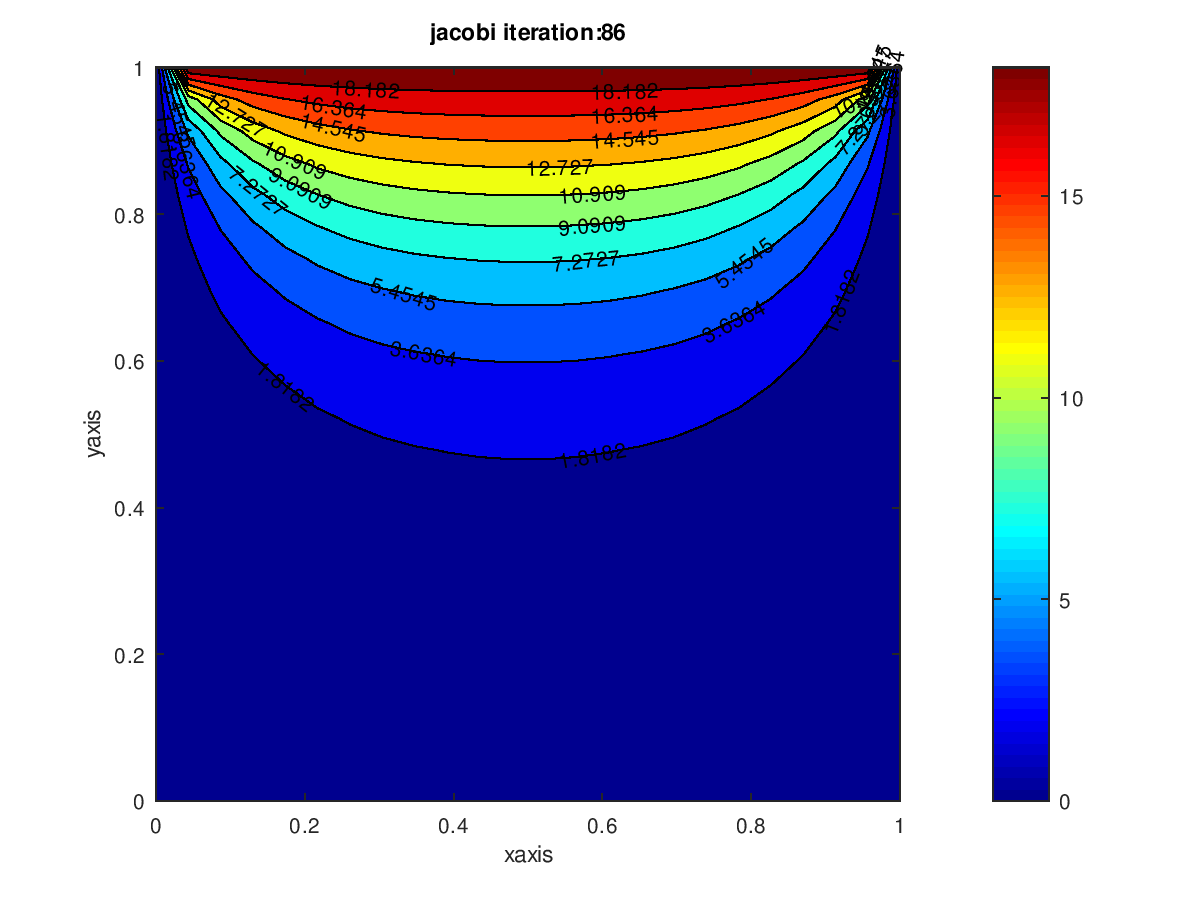
\includegraphics[width=1.0\textwidth]{./static/Jacobi.png}
\caption{Steady state u(x,y)}
\end{figure}
\end{document}
